\documentclass[11pt]{article}

\usepackage[utf8]{inputenc}
\usepackage[T1]{fontenc}
\usepackage[english, french]{babel} %français
\usepackage{amsmath}
\usepackage{amsfonts}
\usepackage{makeidx}
\usepackage{graphicx}
\usepackage[left=2cm,right=2cm,top=2cm,bottom=2cm]{geometry}
\usepackage{mathtools} %dcases
\usepackage{braket} %quantum mechanics
\usepackage[colorlinks=true, linkcolor=black, citecolor=black]{hyperref} % hyperlinks
\usepackage{tikz} % drawing in LaTeX

% the equal sign I use to define something
\newcommand{\define}{\ensuremath{ \overset{\text{def}}{=} }}

% differential element
\renewcommand{\d}[1]{\mathrm{d}#1}

\title{\textbf{Fractal measures and their characterization:} \\ fractal dimensions and the $f-\alpha$ way.}
\author{Nicolas Macé}
\date{31 août 2014}
\begin{document}

\selectlanguage{english}

\maketitle

We consider a topological space $X$, and a (fractal) subspace $F$.
One way of characterizing $F$ is to compute its so-called \emph{Hausdorff dimension}.

\section{Hausdorff dimension and box counting}

In a euclidean space of dimension $d$, balls of radius $l$ have a volume of $l^d$. 
So we expect to need of the order of $1/l^d$ such balls to cover a unit sphere. 
Let us now introduce $N(l)$, the minimal number of (open) balls of radius $l$ needed to cover our subspace $F$. If $N(l)$ scales as $1/l^D$ as $l$ goes to zero, then we say that $D$ is the Hausdorff dimension of $F$.

Sometimes there is no such $D$, ie $N(r)$ does behave as a power law... This happens if $F$ is not a mono fractal, but is a multifractal.
The problem comes from the fact that we limit ourselves to a covering with balls of \emph{uniform} radius. Authorizing now the covering to consist of balls (or equivalently of open sets) of various radii $l_i$ such that  $l_i < l$, we define
\begin{equation}
	H^s(F) \define \lim_{l \rightarrow 0} \inf_{l_i} \Big\{ \sum_i l_i^s \Big| \text{~the balls cover $F$} \Big\} \leq N(l) l^s
\end{equation}
If $s$ is too small, $H^s(F)$ will be infinite. Conversely if $s$ is large enough, $H^s(F)$ is zero. So there is a unique positive $s \define D$ such that 
\begin{equation}
	H^{s < D}(F) = \infty, ~ H^{s > D}(F) = 0
\end{equation}
This $D$ is the Hausdorff dimension of $F$!

This is a great theoretical definition of the Hausdorff dimension, but for practical purposes it appears better to use the following characterization. Consider
\begin{equation}
	\Gamma(\tau,l) \define \sum_i l_i^{-\tau}
\end{equation}
When $l$ goes to zero, there subsists a unique $\tau \define -D$ such that $\Gamma(-D,l)$ does not diverge\footnote{In fact it seems to me that this $D$ is the box-counting dimension rather than the Hausdorff dimension of the set. To do: take $F = \mathbb{Q}$ and see whether using $\Gamma$ we obtain $\tau=0$ (the Hausdorff dimension of $\mathbb{Q}$, a countable set) or $\tau=1$ (the box dimension of $\mathbb{Q}$).}.

\subsection{Computation of the Hausdorff dimension of some (mono)fractals}
For these simple examples, we can take all the balls to be of the same radius $l$. We then have
\begin{equation}
	N(l) \propto \frac{1}{l^D}
\end{equation}
as $l \rightarrow 0$, so that we have $D = \lim_{l\rightarrow 0} \frac{\log N(l)}{\log 1/l}$. 
By a shift of viewpoint, we can imagine having covered $F$ with $N(l)$ \emph{boxes} of length $l$. $N(l)$ is the number of such boxes, and in a space of dimension $d$, $1/l^d$ is their density. \emph{At scale $l$} (ie if the unit of length is $l$), the length of $F$ is $N(l)$. Furthermore if $F$ is embedded in a compact space of unit volume, then 
\begin{equation}
	D = \lim_{l\rightarrow 0} \frac{\log N(l)}{\log N_b^{1/d}}
\end{equation}
where $N_b$ is the number of boxes covering the entire space.

\subsubsection{Cantor set}
We consider the triadic Cantor set, embedded in the unit interval. Because the unit interval is, well, an interval, our boxes are just subintervals of the unit interval.

\begin{itemize}
	\item If the unit of length is 1, the Cantor set has length 1. We have thus obtained $N(1) = 1$.
	\item If the unit of length is $1/3$, the Cantor set has length $2$: $N(1/3) = 2$
	\item Thanks to the fractal nature of the Cantor set, it is easy to see that $N((1/3)^n) = 2^n$.
\end{itemize}
Therefore the Hausdorff dimension of the triadic Cantor set is
\begin{equation}
	D^{\text{Cantor}} = \frac{\log 2}{\log 3}
\end{equation}

\subsubsection{Koch snowflake}

\begin{itemize}
	\item If the unit of length is 1, the snowflake has length 1.
	\item If the unit of length is $1/3$, the snowflake has length 4.
\end{itemize}
Therefore, owing to the fractal nature of this set,
\begin{equation}
	D^{\text{snowflake}} = \frac{\log 4}{\log 3}
\end{equation}

\subsubsection{Sierpinski gasket}
This is a set embedded in the plane! So this time we use 2D boxes, triangularly shaped.
\begin{itemize}
	\item If the unit of surface is 1, the gasket has surface 1.
	\item If the unit of surface is $1/4$, the gasket has surface 3.
\end{itemize}
So, 
\begin{equation}
	D^{\text{gasket}} = \frac{\log 3}{\log 4^{1/2}} = \frac{\log 3}{\log 2}
\end{equation}

\subsubsection{Sierpinski carpet}
This time, we use 2D square-shaped boxes.
\begin{itemize}
	\item If the unit of surface is 1, the gasket has surface 1.
	\item If the unit of surface is $1/9$, the gasket has surface 8.
\end{itemize}
So, 
\begin{equation}
	D^{\text{carpet}} = \frac{\log 8}{\log 9^{1/2}} = \frac{\log 8}{\log 3}
\end{equation}

\subsubsection{Crumpled paper sheet}
Experimentally one can observe the volume of a crumpled sheet of paper scales as
\begin{equation}
	\text{Vol} \propto l^{2.5}
\end{equation}
where $l$ is the length of the paper sheet. So,
\begin{equation}
	D^{\text{crumpled paper}} = 2.5
\end{equation}

\subsection{Box counting overestimates countable sets}
Consider $F = \mathbb{Q}$. Since $\mathbb{Q}$ is a countable set, one can label each of its point, and cover it by a ball. Therefore the number of balls need not increase when $l$ decreases, meaning that the Hausdorff dimension of $\mathbb{Q}$ is zero.

However, if we cover the real line with boxes, every single box contains some points of $\mathbb{Q}$, meaning that the box-counting dimension of this countable set is 1!

In general, adding a contable set to a fractal set $F$ does not affect its Hausdorff dimension, but can very well change the dimension obtained from box counting...

\section{Generalized fractal dimensions}
The Hausdorff dimension can be regarded as one of a number of fractal dimensions, all indexed by an integer, $q$.

Let us cover $F$ with boxes (or balls), and call $p_i$ the total measure in the $i^{\text{th}}$ box. Assuming that $F$ is compact, the total measure of $F$ is normalized to unity: $\sum_i p_i = 1$.
We let
\begin{equation}
	\chi(q) \define \sum_i p_i^q
\end{equation}
As in the previous section, the length of each box $l_i$ is contrained: $l_i < l$. We are interested in the behaviour of $\chi$ in the limit $l \rightarrow 0$.
Obviously $\chi(1) = 1$ and $\chi(0) = N(l) \sim l^{-D}$. In general it turns out that
\begin{equation}
\boxed{
	\chi(q) \sim \text{Cst}~l^{(q-1)D_q}
}
\end{equation}
We also define $\tau(q) \define (q-1) D_q$.

Furthermore we have a local power law behaviour:
\begin{equation}
\boxed{
	p_i^q \sim l^{\alpha_i(q) q}
}
\end{equation}
$\tau(q)$ and $\alpha_i(q)$ completely characterize the fractal behaviour of $F$.

Now that we have defined $\alpha$, we can use it to index the sum appearing in the definition of $\chi$:
\begin{equation}
	\chi(q) \sim \sum_i l^{\alpha_i(q)q} = \sum_\alpha \# \{ \alpha_i(q) | \alpha_i(q) = \alpha\} l^{\alpha q} = \int \d{\alpha} \rho(\alpha) l^{\alpha q - f(\alpha)}
\end{equation}
Where $\d{\alpha'}\rho(\alpha') = \mathbb{P}\{ \alpha \in [\alpha', \alpha' + \d{\alpha'}[ \}$\footnote{Not sure about that one.} and  $\d{\alpha'}\rho(\alpha')l^{-f(\alpha')} = \#\{ \alpha | \alpha \in [\alpha', \alpha' + \d{\alpha'}[  \}$

As $l \rightarrow 0$, only the value of $\alpha$ minimizing $\alpha q - f(\alpha)$ contribute to the integral. We call $\alpha(q)$ this value. We have
\begin{equation}
	\chi(q) \sim l^{\alpha(q) q - f(\alpha(q))}
\end{equation}
and thus
\begin{equation}
\boxed{
	\tau(q) = \alpha(q) q - f(\alpha(q))
}
\end{equation}
We see that $\tau$ is the Legendre transform of a function $f$. We have
\begin{equation}
\boxed{
	f(\alpha(q)) = q \frac{d \tau}{d q}(q) - \tau(q)
}
\end{equation}

\subsection{What can we say about $f$?}
\begin{itemize}
	\item As a Legendre transform, \emph{$f$ must be a convex function of $\alpha$}.
	\item Since $\alpha(0)$ minimizes $- f(\alpha(0))$, \emph{$f$ has a unique maximum at $\alpha(0)$}.
	\item Furthermore $f(\alpha(0)) = D_0$, the Hausdorff dimension.
	\item By definition, $0 \leq \alpha \leq 1$, so that \emph{the graph of $f$ is compact}.
	\item Furthermore $\alpha(+\infty) = D_{+\infty}$, $\alpha(-\infty) = D_{-\infty}$.
\end{itemize}
So, the $f - \alpha$ graph will typically look like
\begin{center}
   	\begin{tikzpicture}[scale=1]
   		
		\draw [->] (-1,0) -- (7,0);
		\draw [->] (0,-1) -- (0,6);
		\filldraw (0.5, 1) circle (0.05) node [below] {$(D_{+\infty},f(\alpha(+\infty)))$};
		\filldraw (4.95, -1) circle (0.05) node [below] {$(D_{-\infty},f(\alpha(-\infty)))$};
		\filldraw (2.5, 5) circle (0.05) node [above] {$(\alpha(0),D_0)$};
		\begin{scope} % limite la portée du clip
			\clip (0.5,-1) rectangle (6,5);
			\draw [domain=0:6, samples=80, smooth] plot (\x, {5 - (2.5-\x)^2}) ;
			\end{scope}
	\end{tikzpicture}
\end{center}
(Not sure if slope must be finite or not at both extremities of the graph)

\subsection{Partition function}

A practical way of computing $f - \alpha$ is to  compute first $\tau - q$ using the so-called \emph{partition function}. Then we can access the $\alpha$ spectrum via $\alpha(q) = \tau'(q)$, and deduce the graph of $f$ on this spectrum using $f(\alpha(q)) = q \alpha(q) - \tau(q)$.

The partition function $\Gamma$ is defined by
\begin{equation}
\boxed{
	\Gamma(q,\tau,l) = \sum_i \frac{p_i^q}{l_i^\tau}
}
\end{equation}
Since $\Gamma > \chi(q)/l^\tau \sim l^{\tau(q) - \tau}$, $\Gamma(\tau < \tau(q)) = 0$, $\Gamma(\tau > \tau(q)) = +\infty$. Only at $\tau = \tau(q)$ does $\Gamma$ have a finite nonzero limit when $l \rightarrow 0$. This gives us a practical way of computing $\tau(q)$.

\subsection{Computation of some $f -\alpha$'s}

\subsubsection{Cantor set}
We construct the triadic Cantor set recursively:
\begin{itemize}
	\item  We start from the unit interval, which has total measure $p_0 = 1$. Thus $\Gamma^{(0)} = 1$.
	\item At step 1, we subdivide $I$ into $[0,1/3]$, $[1/3,2/3]$, $[2/3,1]$. We give the first and the last subintervals measure $p_1 = p_2 = 1/2$. Thus $\Gamma^{(1)} = 2 \frac{(1/2)^q}{(1/3)^\tau}$.
	\item At step $n+1$, $\Gamma^{(n+1)} = \left(\Gamma^{(n)}\right)^2$
\end{itemize}
$\Gamma$ has a finite nonzero limit iff $\Gamma^{(1)} = 1$, that is,
\begin{equation}
\boxed{
	\tau(q) =(q-1) \frac{\log 2}{\log 3}
}
\end{equation}
In particular we recover the Hausdorff dimension $D = \log 2/ \log 3$. We see that the $\alpha$ spectrum consists only of one point: $\alpha(q) = D$. This is typical of a monofractal set.

\subsubsection{Koch snowflake}
As for the Cantor set, $\Gamma^{(n+1)} = \left( \Gamma^{(n)} \right)^2$. 
This time $\Gamma^{(1)} = 4 \frac{(1/4)^q}{(1/3)^\tau}$ and thus
\begin{equation}
\boxed{
	\tau(q) = (q-1)\frac{\log 4}{\log 3}
}
\end{equation}

\subsection{Two scales Cantor set}

\begin{figure}[htp]
\centering
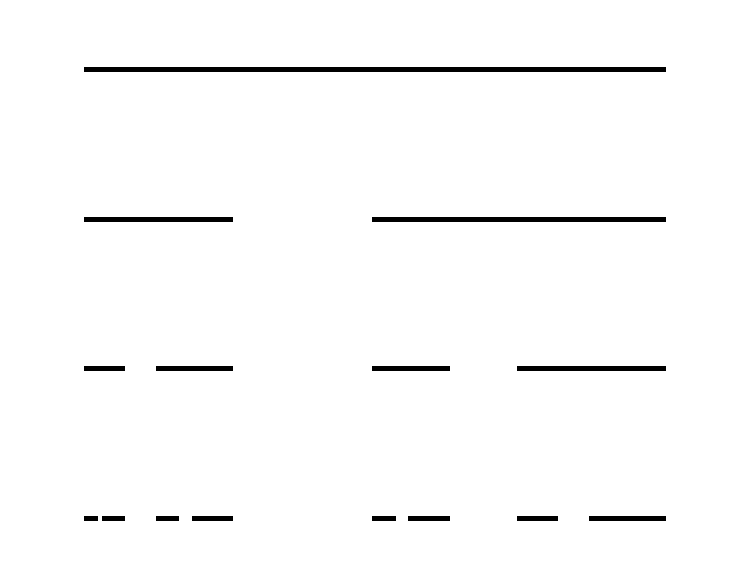
\includegraphics[scale=0.70]{two_scales_cantor_set.pdf}
\caption{Recursive construction of our two scales Cantor set.}
\label{fig:2scal}
\end{figure}

We remove the second quarter of the unit interval. We apply this procedure recursively to the remaining intervals (fig. \eqref{fig:2scal}). 
The limit is a Cantor set, but slightly more complicated than the usual one in the sense that it involves two length scales: $1/2$ and $1/4$.
It has a nontrivial multifractal spectrum!

Because we remove recursively pieces from an inverval, we have again
\begin{equation}
	\Gamma^{(n+1)} = \left( \Gamma^{(n)} \right)^2
\end{equation}
and this time
\begin{equation}
	\Gamma^{(1)} = \frac{\left( \frac{1}{3} \right)^q}{\left( \frac{1}{4} \right)^\tau} + \frac{\left( \frac{2}{3} \right)^q}{\left( \frac{1}{2} \right)^\tau}
\end{equation}
Letting $\tau(q) = \log x(q)/\log 2$ we can transform the equation $\Gamma^{(1)} = 1$ into a second order polynomail equation. We find
\begin{equation}
	x(q) = 2^{q-1} \left( \sqrt{1+ 4 \left( \frac{3}{4} \right)^q} -1 \right)
\end{equation}
Note that in particular the Hausdorff dimension is $\log \tau / \log 2$ where $\tau$ is the golden ratio.

\begin{figure}[htp]
\centering
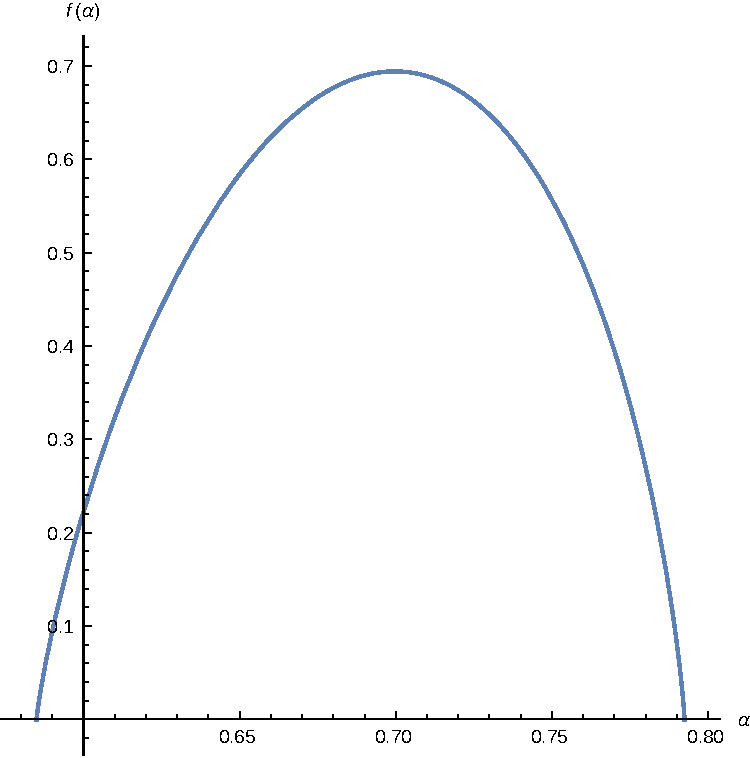
\includegraphics[scale=0.70]{f_alpha_2_scales_cantor_set.pdf}
\caption{$f-\alpha$ graph of the two scales Cantor set.}
\label{fig:falpha2scal}
\end{figure}

This time the $f - \alpha$ graph is nontrivial (fig. \eqref{fig:falpha2scal}).

\subsubsection{Spectrum of the Fibonacci Hamiltonian in the strong quasiperiodicity limit.}

Consider the $n^\text{th}$ approximant of the infinite Fibonacci chain. It is described by a $F_n \times F_n$ Hamiltonian, with periodic boundary conditions. The spectrum of this Hamiltonian consists of $F_n$ energy levels. We label the $i^\text{th}$ level $E^i_n$. At the (periodic) chain level, each $E^i_n$ give rise to a band $\Delta^i_n = |E^i_n(k=0) - E^i_n(k=\pi)|$.

As $n \rightarrow \infty$, $\Delta^i_n \rightarrow 0$. So we can take $\bigcup_i \Delta^i_n$ as a covering for the spectrum of the infinite chain. And $l_i = \Delta^i_n$.
Each box of length $l_i$ has measure $1/F_n$ (as it contains exactly one energy band).

The partition function is thus
\begin{equation}
	\Gamma^{(n)}(q,\tau) = \sum_i \frac{(1/F_n)^q}{\left(\Delta^i_n\right)^\tau}
\end{equation}

In the strong quasiperiodicity limit, we assume that the weak hopping amplitude is far weaker than the strong one: $t_w \ll t_s$.
We can then derive recurrence relations for the band widths \cite{Piechon95}, and from that deduce a recurrence relation on the partition function
\begin{equation}
	\Gamma^{(n)}(q,\tau) = 2 \omega_n^{2q}z^{-\tau}\Gamma^{(n-2)}(q,\tau) + \omega_n^{3q}\bar{z}^{-\tau}\Gamma^{(n-3)}(q,\tau)
\end{equation}
with
\begin{equation}
	\begin{dcases*}
        z = \frac{t_w}{2 t_s}\\
       \bar{z} = \frac{t_w^2}{t_s^2}
     \end{dcases*}
\end{equation}
This recurrence relation is quite different from the one for the triadic Cantor set and the Koch snowflake. 
Requiering that $\Gamma^{(n)}$ has a nonzero limit when $\tau = \tau(q)$, we obtain $\tau(q)$ from an implicit equation:
\begin{equation}
\boxed{
	1 = 2 \omega^{2q} z^{-\tau(q)} + \omega^{3q} \bar{z}^{-\tau(q)}
}
\end{equation}
In particular, when $z = \bar{z}^{2/3}$, that is when $t_s = 8 t_w$, we have
\begin{equation}
	\tau(q) = (q-1)\frac{\log \omega^{-1}}{\log 4}
\end{equation}
This is the only ratio of the couplings for which the fractal is a monofractal!
\bibliography{fractal_measures.bib}{}
\bibliographystyle{plain}
\end{document}